\documentclass{article}

\usepackage{amsmath}
\usepackage{float}
\usepackage{graphicx}

\usepackage[colorlinks=true, allcolors=blue]{hyperref}

\title{Lista 1}
\author{Luís Felipe Ramos Ferreira}
\date{\href{mailto:lframos.lf@gmail.com}{\texttt{lframos.lf@gmail.com}}
}

\begin{document}

\maketitle

\begin{enumerate}

	\item Capítulo lido
	      %imagem de trabalho feito
	\item
	      \begin{itemize}
		      \item (1.5.3)
		            \begin{enumerate}
			            \item
			                  A seguinte argumentação pode ser feita para provar a igualdade usando contagem dupla.
			                  Olhando para o lado esquerdo, sabemos que \(\binom{n}{k} \binom{k}{m}\) representa o número de maneira de escolher
			                  um conjunto \(S\) de \(k\) elementos dentre \(n\) elementos, e depois escolher um conjunto \(S'\) subconjunto de \(S\) com \(m\)
			                  elementos. Somando esse valor onde \(k\) varia de \(m\) até \(n\) retorna o número de maneiras de fazer a divisão em conjuntos citada
			                  de modo que o conjunto \(S'\) final tenha tamanho \(m\).
			                  Podemos ntoar que o conjunto \(S'\) de tamanho \(m\) pode ser escolhido de \(\binom{n}{m}\) diferentes.
			                  Dessas maneiras, podemos escolher \(2^{n - m}\) subconjutnos dos \(n\) elementos originais que não estão em \(S'\). Logo, existem
			                  \(2^{n - m} \binom{n}{m}\) maneiras de fazer a divisão. Portanto, ambos lados da equação são iguais.
			                  Podemos usar também um argumento algébrico nessa questão.

			                  \begin{figure}[H]
				                  \centering
				                  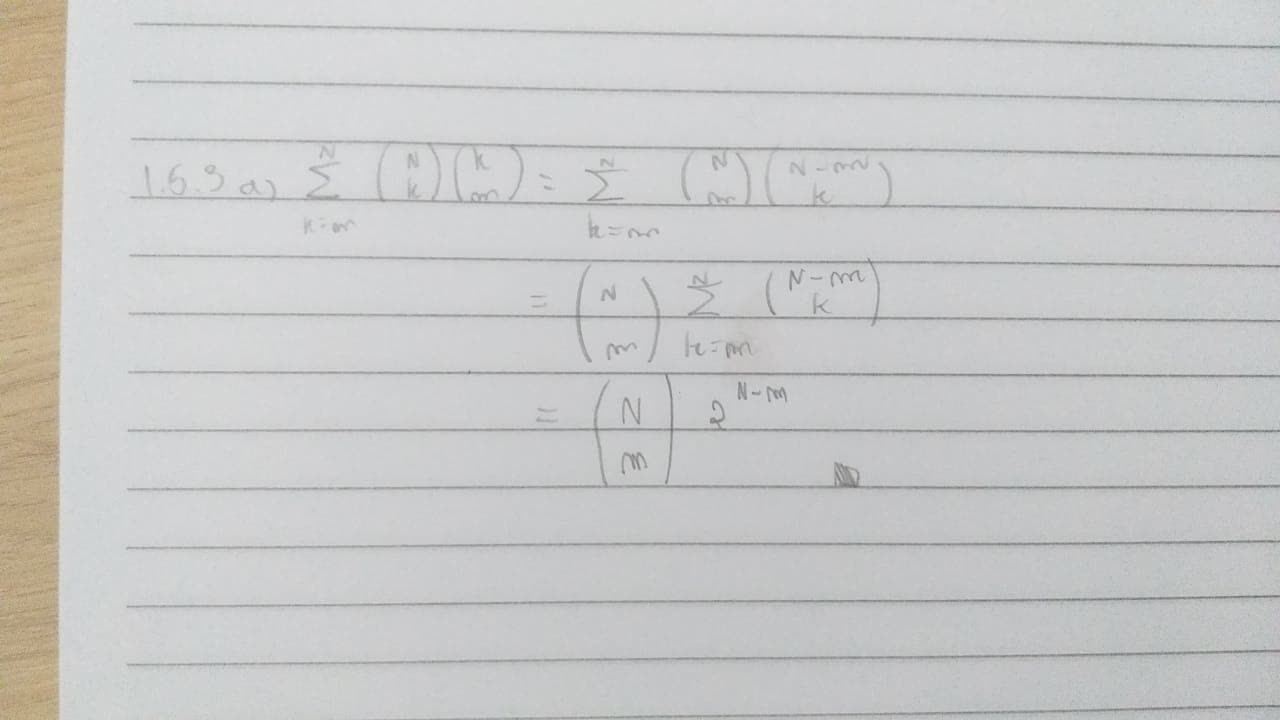
\includegraphics[width=0.8\textwidth]{images/153a.jpeg}
				                  \caption{Questão 1.5.3 - a)}
			                  \end{figure}
			            \item
			                  OK Do lado esquerdo, temos \(\binom{n}{m} \binom{m}{k}\). Sabemos que \(\binom{n}{m}\) representa o número de subconjuntos de tamanho \(m\) de um conjunto com
			                  \(n\) elementos. Por sua vez, \(\binom{m}{k}\) representa o número de subconjuntos de tamanho \(k\) de um conjunto com \(m\) elementos. Desse modo, esse produto representa o número de maneiras de escolher \(k\) elementos de um conjunto de \(m\) elementos que foram previamente escolhidos de um conjunto de \(n\) elementos.
			                  Do lado direito da equação, temos \(\binom{n}{k} \binom{n - k}{m - k}\). Sabemos que \(\binom{n}{k}\) representa o número de subconjuntos de tamanho \(k\) de um conjunto de tamanho \(n\). \(\binom{n-k}{m-k}\), por sua vez, é o número de conjuntos de tamanho \(m-k\) de um conjunto de tamanho \(n-k\). O produto final então é o número de subconjuntos de tamanho \(k\) de um subconjunto de tamanho \(m\) escolhido de um conjunto de tamanho \(n\), assim como no lado esquerdo. Como ambos os lados representam o mesmo valor combinatório, eles são iguais.
			                  Uma prova algébrica também pode ser obtida como visto abaixo.
			                  \begin{figure}[H]
				                  \centering
				                  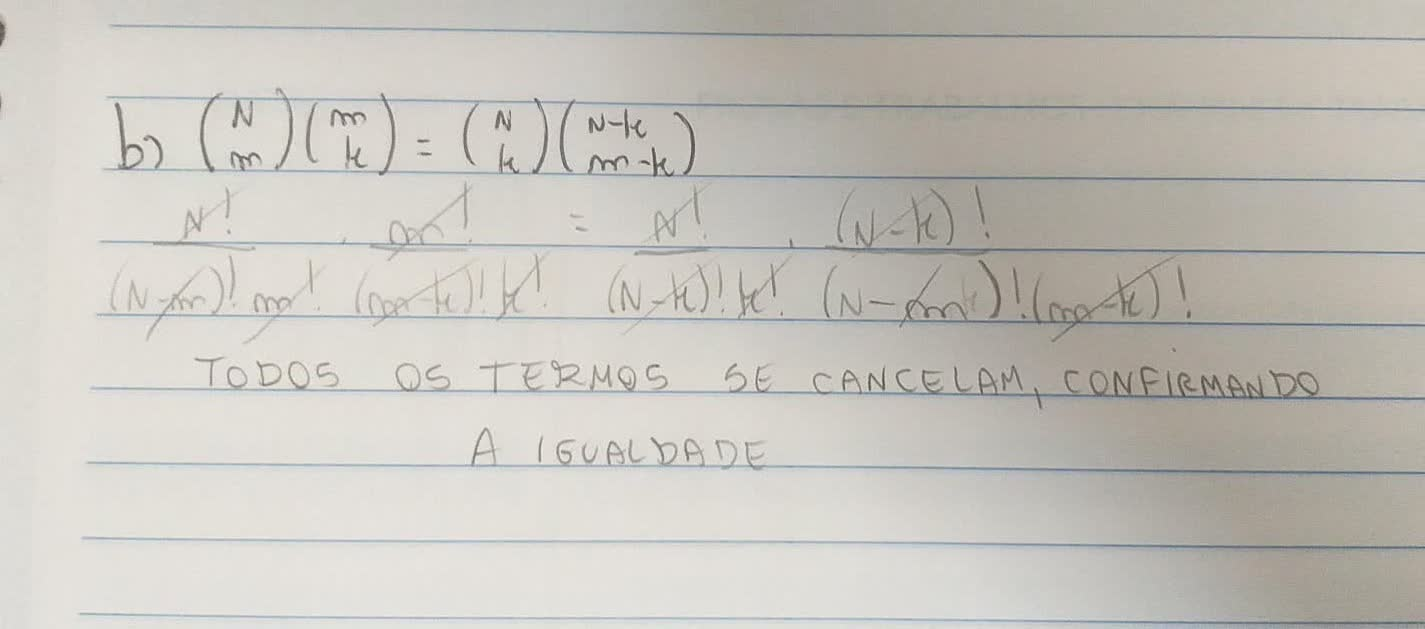
\includegraphics[width=0.8\textwidth]{images/153b.jpg}
				                  \caption{Questão 1.5.3 - b)}
			                  \end{figure}
			            \item
			                  Podemos pensar numa solução para esse problemas utilizando contagem dupla da seguinte forma.
			                  Suponha que estamos escolhendo livros de uma livraria. O lado direito da equação, \(\binom{n + 1}{m + 1}\), conta
			                  diretamente de quantas maneiras podemos escolher \(m + 1\) livros de uma livraria com \(n + 1\) livros.
			                  O lado esquerdo da equação \(\sum_{k=m}^{n} \binom{k}{m}\), pode ser interpretado da seguinte maneira.
			                  Vamos supor que o último livro escolhido foi enumerado com o valor \(k + 1\). Logo, os \(m\) livros que ainda não tiveram um valor atribuído a eles
			                  devem ter um valor escolhido entre \(1\) e \(k\) e, combinatoriamente, existem \(\binom{k}{m}\) maneiras de fazer isso.
			                  Como \(k\) pode ter qualquer valor entre \(m\) e \(n\) e somarmos esse valor, teremos a parte da esquerda da expressão.
			                  Essa igualdade também pode ser demonstrada algebricamente, como visto na imagem abaixo.
			                  \begin{figure}[H]
				                  \centering
				                  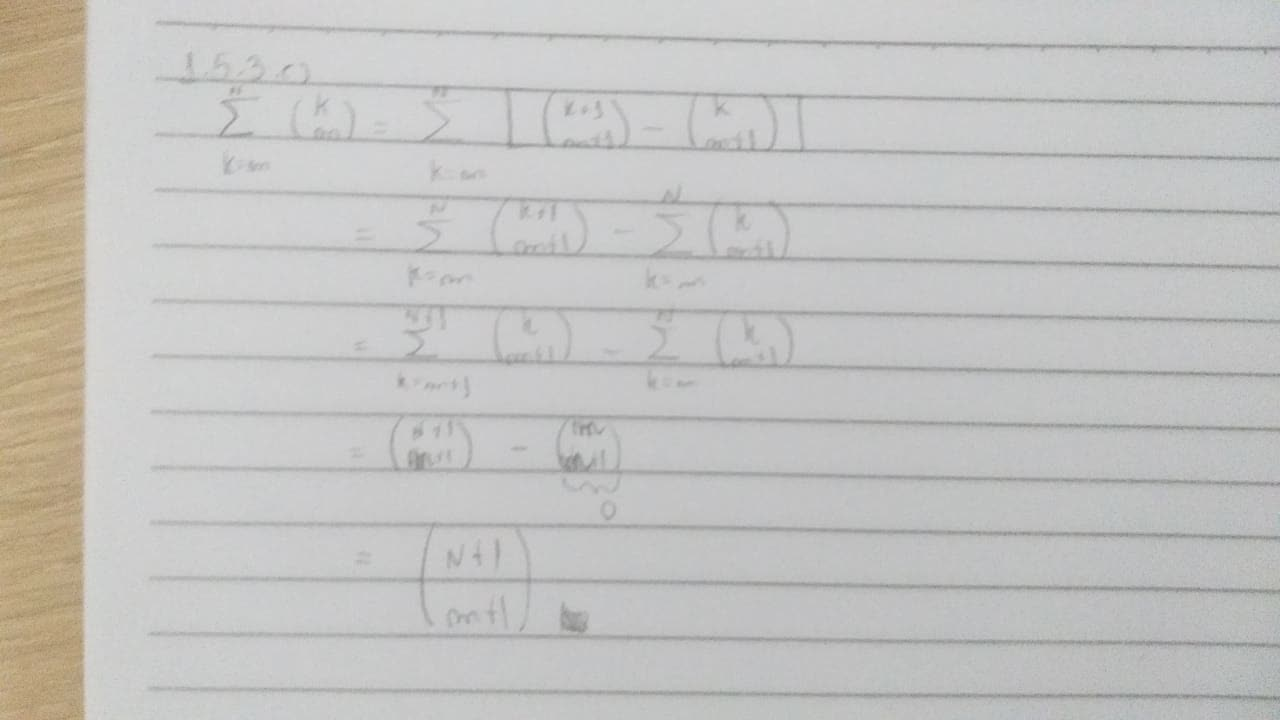
\includegraphics[width=0.8\textwidth]{images/153c.jpeg}
				                  \caption{Questão 1.5.3 - c)}
			                  \end{figure}
		            \end{enumerate}
		      \item OK (1.5.6) Seja \(G\) um grafo qualquer com \(n\) vértices. Suponha, por contradição, que não existam dois vértices em \(G\) com o mesmo grau. Logo, como existem \(n\) vértices no grafo, os \(n\) possíveis graus que um vértice pode ter são \(\{0, 1, \dots, n-1\}\), logo podemos dizer que estes são os graus dos vértices de \(G\). No entanto, isso é absurdo, pois existiram um vértice de grau 0 e um vértice de grau \(n-1\) em um grafo com \(n\) vértices, o que não faz sentido. Logo, a premisa inicial estava errada, e podemos afirmar que todo grafo com \(n\) vértices, \(n \geq 2\), possui dois vértices com o mesmo grau.
		      \item (1.5.11) indução?
	      \end{itemize}
	\item \begin{itemize}
		      \item OK (2.8.3) Seja \(G\) um grafo com número cromático igual a \(\mathcal{X}(G)\). Sabemos que, para qualquer par de cores \(c_1, c_2\) da coloração mínima, deve existir ao menos uma aresta entre vértices \(v_1\), com cor \(c_1\), e \(v_2\), com cor \(c_2\). Caso contrário, todos os vértices com cor \(c_2\), poderiam ser coloridas com a cor \(c_1\) (sem perda de generalidade), o que seria contraditório com o fato da coloração ser mínima. Logo, para cada par de cores na coloração, deve existir ao menos uma aresta, e como cada aresta conecta exatamente dois vértices, temos que \(e(G) \ge \binom{\mathcal{X}(G)}{2}\).
		      \item OK (2.8.9) Seja \(G\) um grafo bipartido. Pelo teorema de Kõnig, o tamanho do emparelhamento máximo em \(G\) é
		            igual ao tamanho do conjunto de cobertura por vértices (\textit{vertex cover}) mínimo de \(G\). Sabemos que o
		            tamanho do \textit{vertex cover} mínimo é com certeza maior do que \(\frac{e(G)}{\Delta(G)}\). Note que o \textit{vertex cover} cobre todas as
		            arestas do grafo, sendo que cada vértice \(v\) nele cobre no máximo \(\Delta(G)\) arestas. Portanto, se multiplicarmos \(\beta(G)\) , que é
		            o tamanho do \textit{vertex cover} mínimo, por \(\Delta(G)\), obteremos um número maior que \(e(G)\). Logo, concluímos a afirmação.
		            Algebricamente temos a seguinte prova:

		            \[M(G) = \beta(G) \geq \frac{e(G)}{\Delta(G)}\]
		            \[\beta(G)\Delta(G) \geq e(G)\]


		      \item OK (2.8.15) A prova será feita considerando uma indexação diferente da usada no livro. Isso não altera a semântica do problema.
		            Provaremos que se \(k \in \mathcal{N}\) e \(T\) é uma árvore cm \(k\) vértices,
		            então \(T\) é subárvore de qualquer grafo \(G\) com \(\delta(G) \geq k\).
		            A prova por ser feita por indução no número de arestas da árvore. A solução é trivial para o caso base em que \(e(T) = 1\). Para \(e(T) = 1\), \(T\) é uma aresta e trivialmente é subgrafo de qualquer grafo \(G\) com \(\delta(G) \geq 1\). Suponha que o resultado vale para qualquer árvore com \(k\) arestas, \(k > 1\)
		            . Seja \(T\) uma árvore qualquer com \(k + 1\) arestas e \(T' = T - \{v\}\) para alguma folha \(v \in V(T)\) e seja \(w\) o vizinho de \(v\) em \(T\), que com certeza
		            existe e é único já que \(v\) é uma folha.
		            Pela hipótese indutiva, sabemos que \(T'\) é um subgrafo de todo
		            grafo \(G\) tal que \(\delta(G) = k+1\). Como o grau de \(w\) em \(G\) é
		            maior ou igual a \(k + 1\) e \(T'\) possui \(k - 1\) vértices diferentes de \(v\),
		            podemos afirmar que existe um vizinho de \(w\) em \(G\) que não está em \(T'\). Escolhemos esse vértice, vamos denotá-lo
		            por \(l\). Adicionamos a aresta \(wl\) à \(T'\) para obter uma árvore isomorfa à \(T\) em \(G\). Demonstramos então que se a afirmativa é verdade para
		            uma árvore com \(k\) arestas, então também é verdade para uma árvore com \(k + 1\) arestas,
		            o que conclui a prova do teorema.
	      \end{itemize}

	\item

	      \begin{itemize}
		      \item (3.5.1)
		            Primeiramente, mostraremos que \(ex(m, K_{k + 1}) \leq (1 - \frac{1}{n})\frac{n^2}{2}\).
		            A prova será feita por indução em \(n\). No caso base, considere
		            \(n \leq k\). Desse modo, temos que \(ex(n, K_{k + 1}) = \binom{n}{2} \leq t_k\).
		            Seja agora \(G\) um grafo com \(n > k\) vértices, livre de
		            \(K_{k + 1}\), tal que o número de arestas em \(G\) está maximizado.
		            Sabemos que \(G\) possui um \(K_k\) como subgrafo, pois caso contrário a adição de uma aresta não introduziria
		            um \(K_{k + 1}\) no grafo e isso aumentaria o número de arestas dele, um absurdo pois assumimos que o número de arestas era máximo.

		            Seja agora \(H = G - K_k\). Pela hipótese, \(|E(H)| \leq (1 - \frac{1}{n})\frac{n^2}{2}\).
		            Logo temos que \(|E(G)| \leq (1 - \frac{1}{n})\frac{n^2}{2} + (n-k)(k-1) + \binom{n}{2}\),
		            como queríamos demonstrar.

		      \item (3.5.5)
		            %  e(g) > n^2/4  then g has at least floor(n/2) triangles
		            % 			for n = 1, 2, 3 trivial
		            %    				suppose true for k
		            % 			lets show for k+1
		            %    				suppose k+1 is even
		            %    				let v be an arbitrary vertex of g, remove it
		            % G - v has at least (k-1)/2 triangs. Adding v

		      \item (3.5.6)
		      \item (3.5.7)
		      \item (3.5.8)
		      \item (3.5.9)
	      \end{itemize}
\end{enumerate}

\end{document}
